\documentclass[aspectratio=169,10pt]{beamer}
\usetheme[progressbar=frametitle,numbering=fraction,block=fill]{metropolis}
\usepackage{fontspec}
\setsansfont{Lato}[Path=/usr/share/fonts/truetype/lato/,Extension=.ttf,UprightFont=*-Regular,BoldFont=*-Bold,ItalicFont=*-Italic,BoldItalicFont=*-BoldItalic]
\setmonofont{DejaVu Sans Mono}[Scale=0.8]
\usepackage[spanish,es-tabla,es-nodecimaldot]{babel}
\usepackage{graphicx,booktabs,tikz}
\usetikzlibrary{arrows.meta,positioning}
\graphicspath{{figuras/}}
% generado por pruebas/conftest.py: no editar a mano
\newcommand{\PruebasOk}{77}
\newcommand{\PruebasTotal}{81}
\newcommand{\PruebasFallan}{4}


% ---------- paleta verde
\definecolor{verde}{HTML}{0B5D45}
\definecolor{verde2}{HTML}{14A37F}
\definecolor{verdeclaro}{HTML}{E6F4EF}
\definecolor{ambar}{HTML}{E0962A}
\definecolor{rojo}{HTML}{C0392B}
\definecolor{gris}{HTML}{5C6D7E}
\setbeamercolor{frametitle}{bg=verde,fg=white}
\setbeamercolor{progress bar}{fg=verde2,bg=verde!25}
\setbeamercolor{title separator}{fg=verde2}
\setbeamercolor{progress bar in head/foot}{fg=verde2,bg=verde!25}
\setbeamercolor{progress bar in section page}{fg=verde2,bg=verde!25}
\setbeamercolor{alerted text}{fg=verde2}
\setbeamercolor{block title}{bg=verde,fg=white}
\setbeamercolor{block body}{bg=verdeclaro,fg=black}
\setbeamercolor{block title alerted}{bg=rojo,fg=white}
\setbeamercolor{block body alerted}{bg=rojo!8,fg=black}
\setbeamercolor{background canvas}{bg=white}
\setbeamercolor{normal text}{fg=black!85}
\setbeamercolor{section in toc}{fg=verde}
\setbeamertemplate{itemize item}{\textcolor{verde2}{\rule[.2ex]{.9ex}{.9ex}}}
\setbeamertemplate{itemize subitem}{\textcolor{verde2}{--}}

\newcommand{\cifra}[2]{\begin{center}{\fontsize{30}{32}\selectfont\bfseries\color{verde}#1}\\[2pt]{\small\color{gris}#2}\end{center}}
\newcommand{\sint}{{\scriptsize\color{gris}\itshape Datos sintéticos (simulación SUMO), no medidas de campo.}}
\newcommand{\quien}[1]{\hfill{\footnotesize\color{gris}#1}}

\title{Centro de tráfico predictivo para Cuenca}
\subtitle{Predicción a 1 hora, detección de incidentes y aviso V2X validado en SUMO}
\author{Angel Apolo \and Fernando Terán \and Stalyn Ochoa \and Karla Barrera}
\institute{Redes Vehiculares · Proyecto Interciclo · Universidad de Cuenca}
\date{}

\begin{document}

\maketitle

% ================= ANGEL
\begin{frame}{El problema en una frase}
\vspace{4pt}
\begin{center}
{\Large Cuando un accidente cierra una avenida de Cuenca, \alert{nadie lo sabe hasta que la cola ya creció}, y los autos que vienen detrás siguen entrando a ella.}
\end{center}
\vspace{8pt}
\begin{columns}[T]
\begin{column}{.5\textwidth}
\small Queremos que un centro de tráfico:
\begin{enumerate}
\item \alert{prevea} cómo estará la ciudad en 1 hora,
\item \alert{detecte} el accidente en minutos,
\item \alert{avise} por V2X (DENM) a los autos que van hacia allá.
\end{enumerate}
\end{column}
\begin{column}{.45\textwidth}
\begin{block}{Metas del curso}
\small Predicción: MAE < 3 km/h\\
Detector: DR ≥ 85 \%, MTTD < 5 min, FAR 3–5 \%\\
Aviso: mejora medida en SUMO
\end{block}
\end{column}
\end{columns}
\end{frame}

\begin{frame}{El lazo completo: dato, modelo, acción, medida y visualización}
\centering
\begin{tikzpicture}[font=\sffamily\small,
  c/.style={draw=verde,fill=verdeclaro,rounded corners=4pt,minimum height=1.85cm,align=center,text width=2.1cm},
  f/.style={-{Latex[length=2mm]},thick,draw=verde}]
\node[c] (d) {\textbf{Dato}\\[2pt]\scriptsize detectores por carril y autos V2X};
\node[c,right=.42cm of d] (m) {\textbf{Modelo}\\[2pt]\scriptsize GCN-GRU (1 h) y detector de incidentes};
\node[c,right=.42cm of m] (a) {\textbf{Acción}\\[2pt]\scriptsize DENM a autos V2X a < 2 km: cambian de ruta};
\node[c,right=.42cm of a] (me) {\textbf{Medida}\\[2pt]\scriptsize SUMO mide demora, cola y viajes};
\node[c,right=.42cm of me] (v) {\textbf{Visualización}\\[2pt]\scriptsize tablero web en vivo};
\draw[f] (d)--(m); \draw[f] (m)--(a); \draw[f] (a)--(me); \draw[f] (me)--(v);
\draw[f] (me.south) |- ++(0,-.55) -| node[pos=.25,below,font=\scriptsize\sffamily]{el tráfico cambia y el detector vuelve a medir: bucle cerrado con TraCI, minuto a minuto} (d.south);
\end{tikzpicture}
\vspace{14pt}
\begin{itemize}\small
\item Todo corre sobre un \alert{gemelo digital de Cuenca} en SUMO: los datos son sintéticos, justificados y reproducibles
\item El mismo día se simula dos veces, \alert{con y sin la IA}: así se mide qué cambia la acción
\end{itemize}
\end{frame}

\begin{frame}{Dato: gemelo digital de Cuenca con datos sintéticos justificados}
\begin{columns}[c]
\begin{column}{.5\textwidth}
\footnotesize
\begin{itemize}
\item Red real de OpenStreetMap (15 parroquias urbanas), \alert{SUMO 1.12}
\item \alert{66 días} simulados, \textasciitilde190\,000 viajes por día, con lluvia y fines de semana
\item 1694 celdas de 200 m y 310 tramos con detectores en Américas, Circunvalación Sur y Remigio Crespo
\item Dos vistas: sensores (todos los autos) y \alert{V2X 50 \%}
\end{itemize}
\begin{block}{Por qué sintéticos y cómo se justifican}
\scriptsize No hay datos de la EMOV para este periodo. Generador documentado (duarouter, semilla = 1000 + día), parámetros con fuente publicada y \alert{validación} contra datos reales de Cuenca (anexo del informe). El código acepta el dato real con el mismo formato.
\end{block}
\end{column}
\begin{column}{.48\textwidth}
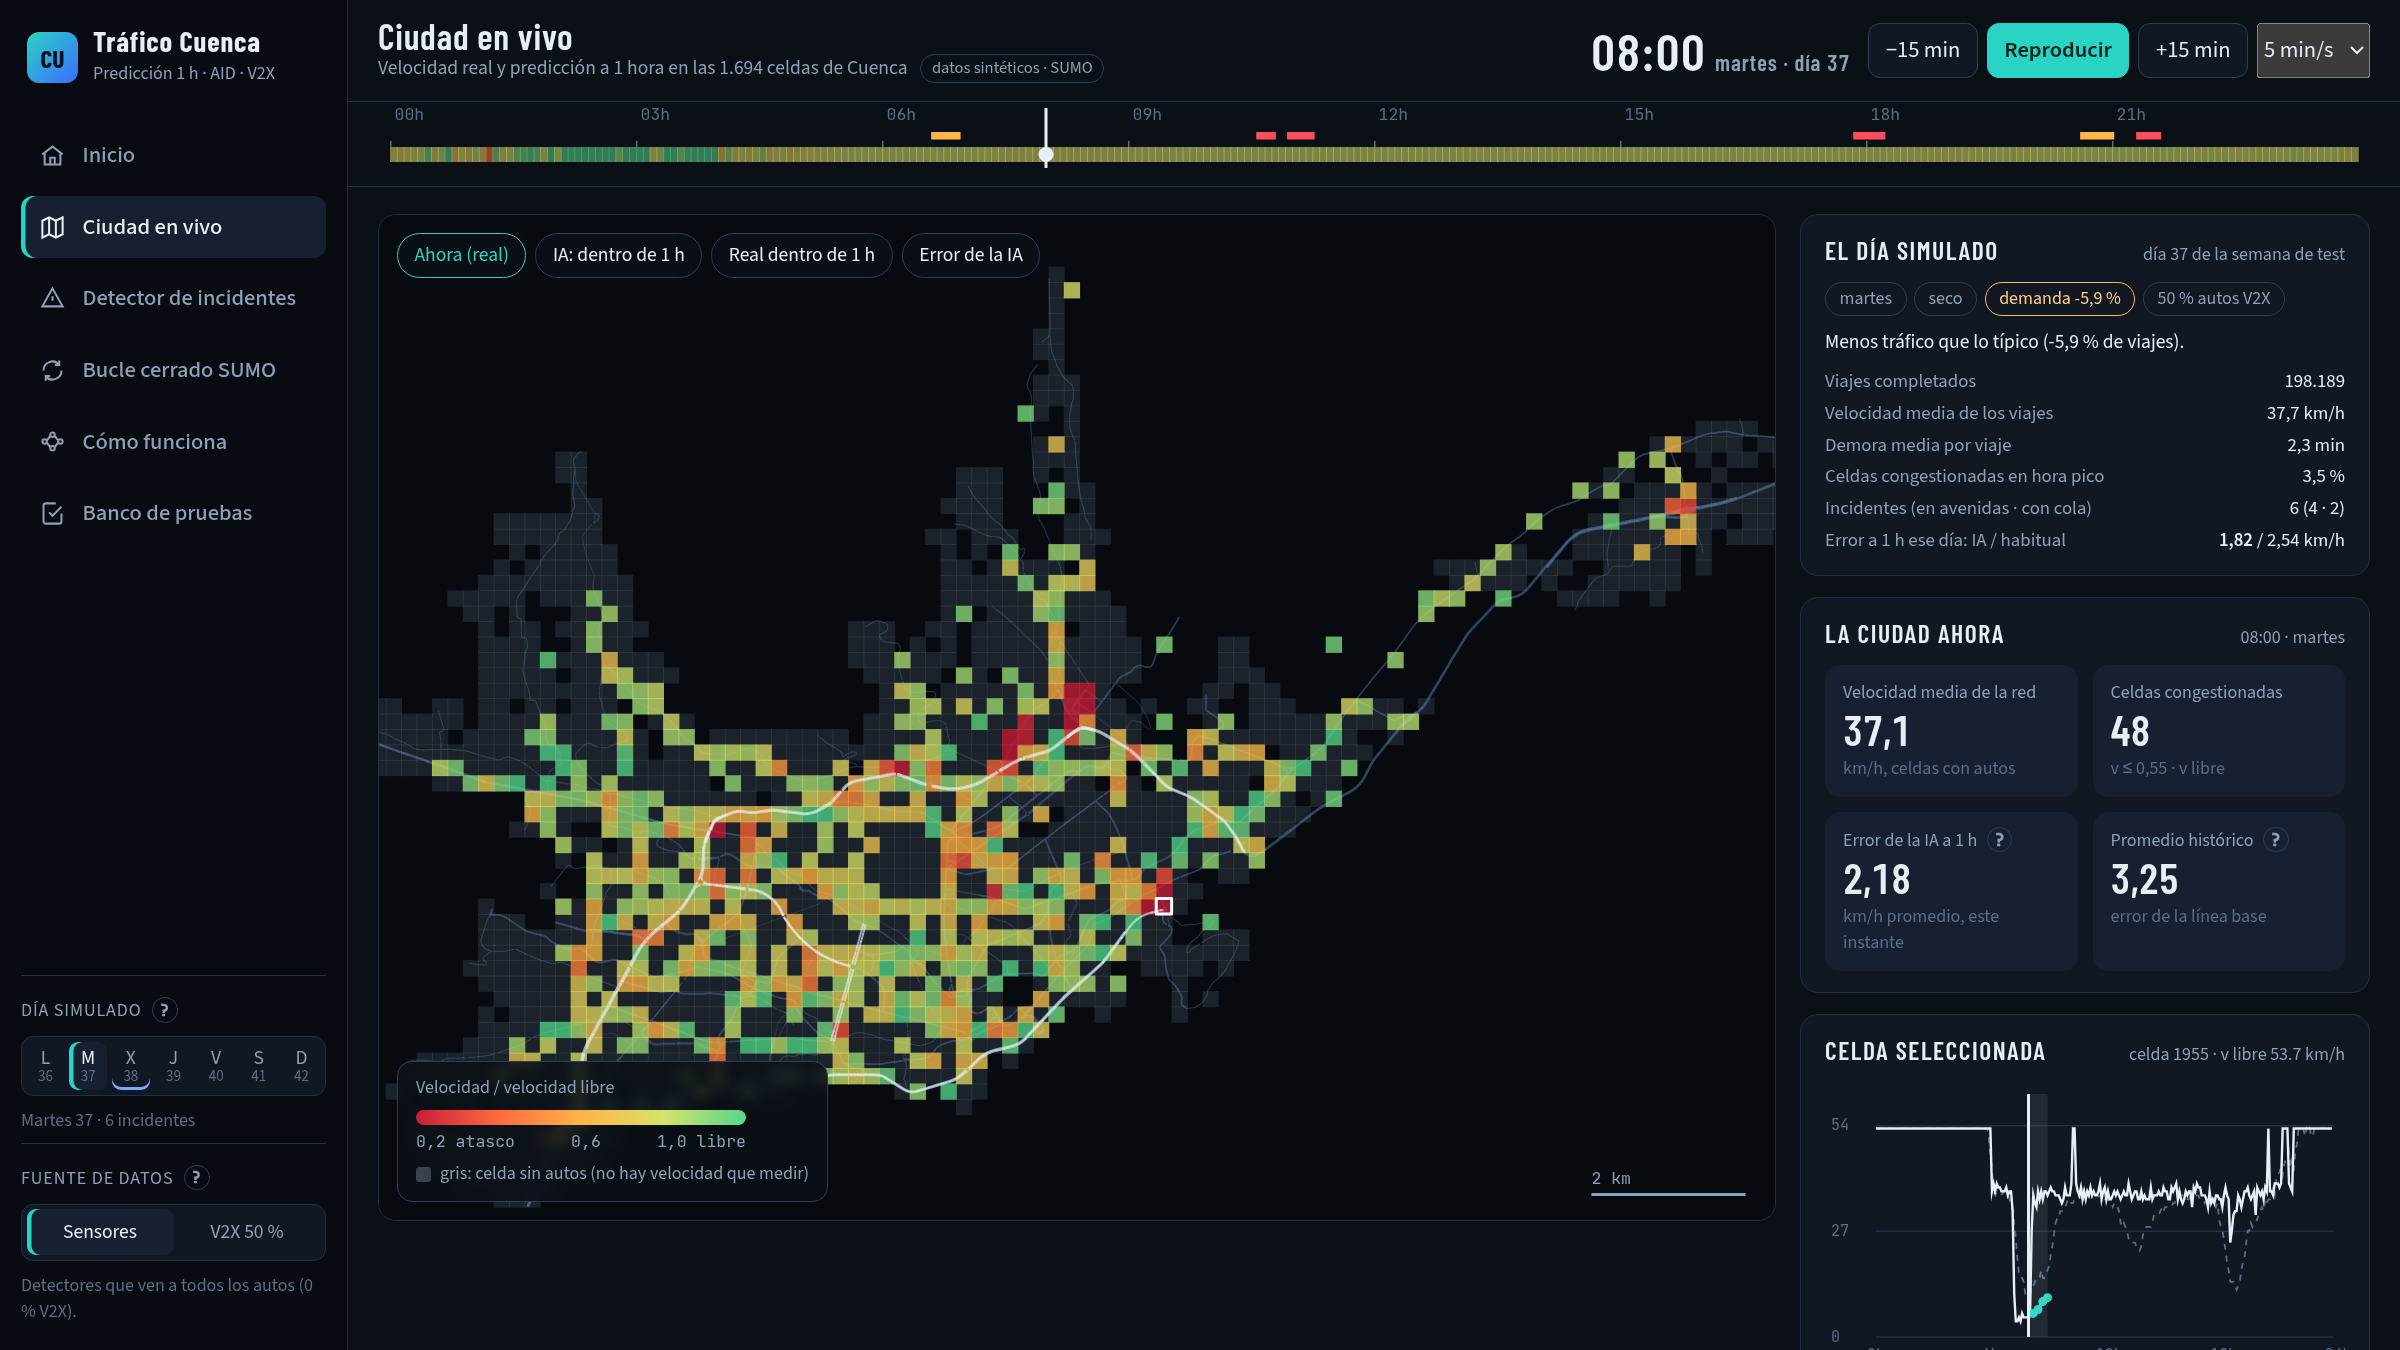
\includegraphics[width=\textwidth]{dash_ciudad_real.png}\\[-2pt]
\sint
\end{column}
\end{columns}
\end{frame}

% ================= FERNANDO
\begin{frame}{Modelo 1: predecir la ciudad dentro de una hora}
\centering
\begin{tikzpicture}[font=\sffamily\small,
  c/.style={draw=verde,fill=verdeclaro,rounded corners=3pt,minimum height=1.05cm,align=center,text width=2.3cm},
  f/.style={-{Latex[length=2mm]},thick,draw=verde}]
\node[c] (in) {1 hora de historia\\12 pasos × 6 canales};
\node[c,right=.55cm of in] (g) {Grafo de calles\\aguas arriba y abajo};
\node[c,right=.55cm of g] (r) {GRU\\memoria de 1 h};
\node[c,right=.55cm of r] (o) {Corrección\\+15 … +60 min};
\node[c,below=.6cm of o,fill=ambar!15,draw=ambar] (ha) {Promedio histórico\\(lo habitual)};
\node[c,below=.6cm of r,fill=white] (y) {Velocidad\\predicha};
\draw[f] (in)--(g); \draw[f] (g)--(r); \draw[f] (r)--(o); \draw[f] (o)--(y); \draw[f,draw=ambar] (ha)--(y);
\end{tikzpicture}
\vspace{6pt}
\begin{itemize}\small
\item Lo habitual ya explica la rutina; la red aprende \alert{qué será distinto hoy} (lluvia, incidente, día cargado)
\item Liviana: \alert{29\,908 parámetros}, entrena en CPU
\item Con V2X: conteos divididos por la penetración (50 \%)
\end{itemize}
\end{frame}

% ================= STALYN
\begin{frame}{Modelo 2: ¿accidente u hora pico?}
\begin{columns}[c]
\begin{column}{.56\textwidth}
\small
\begin{itemize}
\item \alert{Desvío de lo habitual}: ¿es raro para este tramo a esta hora?
\item \alert{Firma espacial}: cola antes y vía vacía después (idea del algoritmo California)
\item \alert{Contexto}: si toda la ciudad está lenta, es lluvia
\item \alert{Novedad}: un accidente es un cambio brusco
\item Gradient Boosting con 39 rasgos; alarma tras 3 min seguidos
\end{itemize}
\end{column}
\begin{column}{.4\textwidth}
\begin{block}{Umbral sin mirar el test}
\small Elegido en 51 días de entrenamiento y validación, con FAR ≤ 3 \%; umbral aparte con lluvia.
\end{block}
\begin{block}{Datos para el detector}
\small 20 días extra con 8 incidentes cada uno: 132 de 271 forman cola.
\end{block}
\end{column}
\end{columns}
\end{frame}

\begin{frame}{Acción: la IA dentro de SUMO, minuto a minuto}
\centering
\begin{tikzpicture}[font=\sffamily\small,
  c/.style={draw=verde,fill=verdeclaro,rounded corners=3pt,minimum height=1cm,align=center,text width=2.4cm},
  f/.style={-{Latex[length=2mm]},thick,draw=verde}]
\node[c] (s) {SUMO\\día 119, cierre total};
\node[c,right=.6cm of s] (d) {Detectores\\TraCI cada 1 s};
\node[c,right=.6cm of d] (a) {Detector de\\incidentes cada min};
\node[c,right=.6cm of a] (m) {DENM\\autos V2X a < 2 km};
\draw[f] (s)--(d); \draw[f] (d)--(a); \draw[f] (a)--(m);
\draw[f] (m.south) |- ++(0,-.55) -| node[pos=.25,below,font=\scriptsize\sffamily]{el navegador del auto recalcula con el tráfico actual} (s.south);
\end{tikzpicture}
\vspace{12pt}
\begin{itemize}\small
\item Dos corridas \alert{idénticas} (misma demanda y semilla): sin IA y con IA
\item Aviso realista: área de 2 km, +10 min de penalización al tramo, \alert{caduca a los 3 min} sin alarma
\item Umbral estricto (FAR ≤ 1 \%) para no desviar autos por falsas alarmas
\end{itemize}
\end{frame}

% ================= KARLA
\begin{frame}{Demo en vivo}
\centering
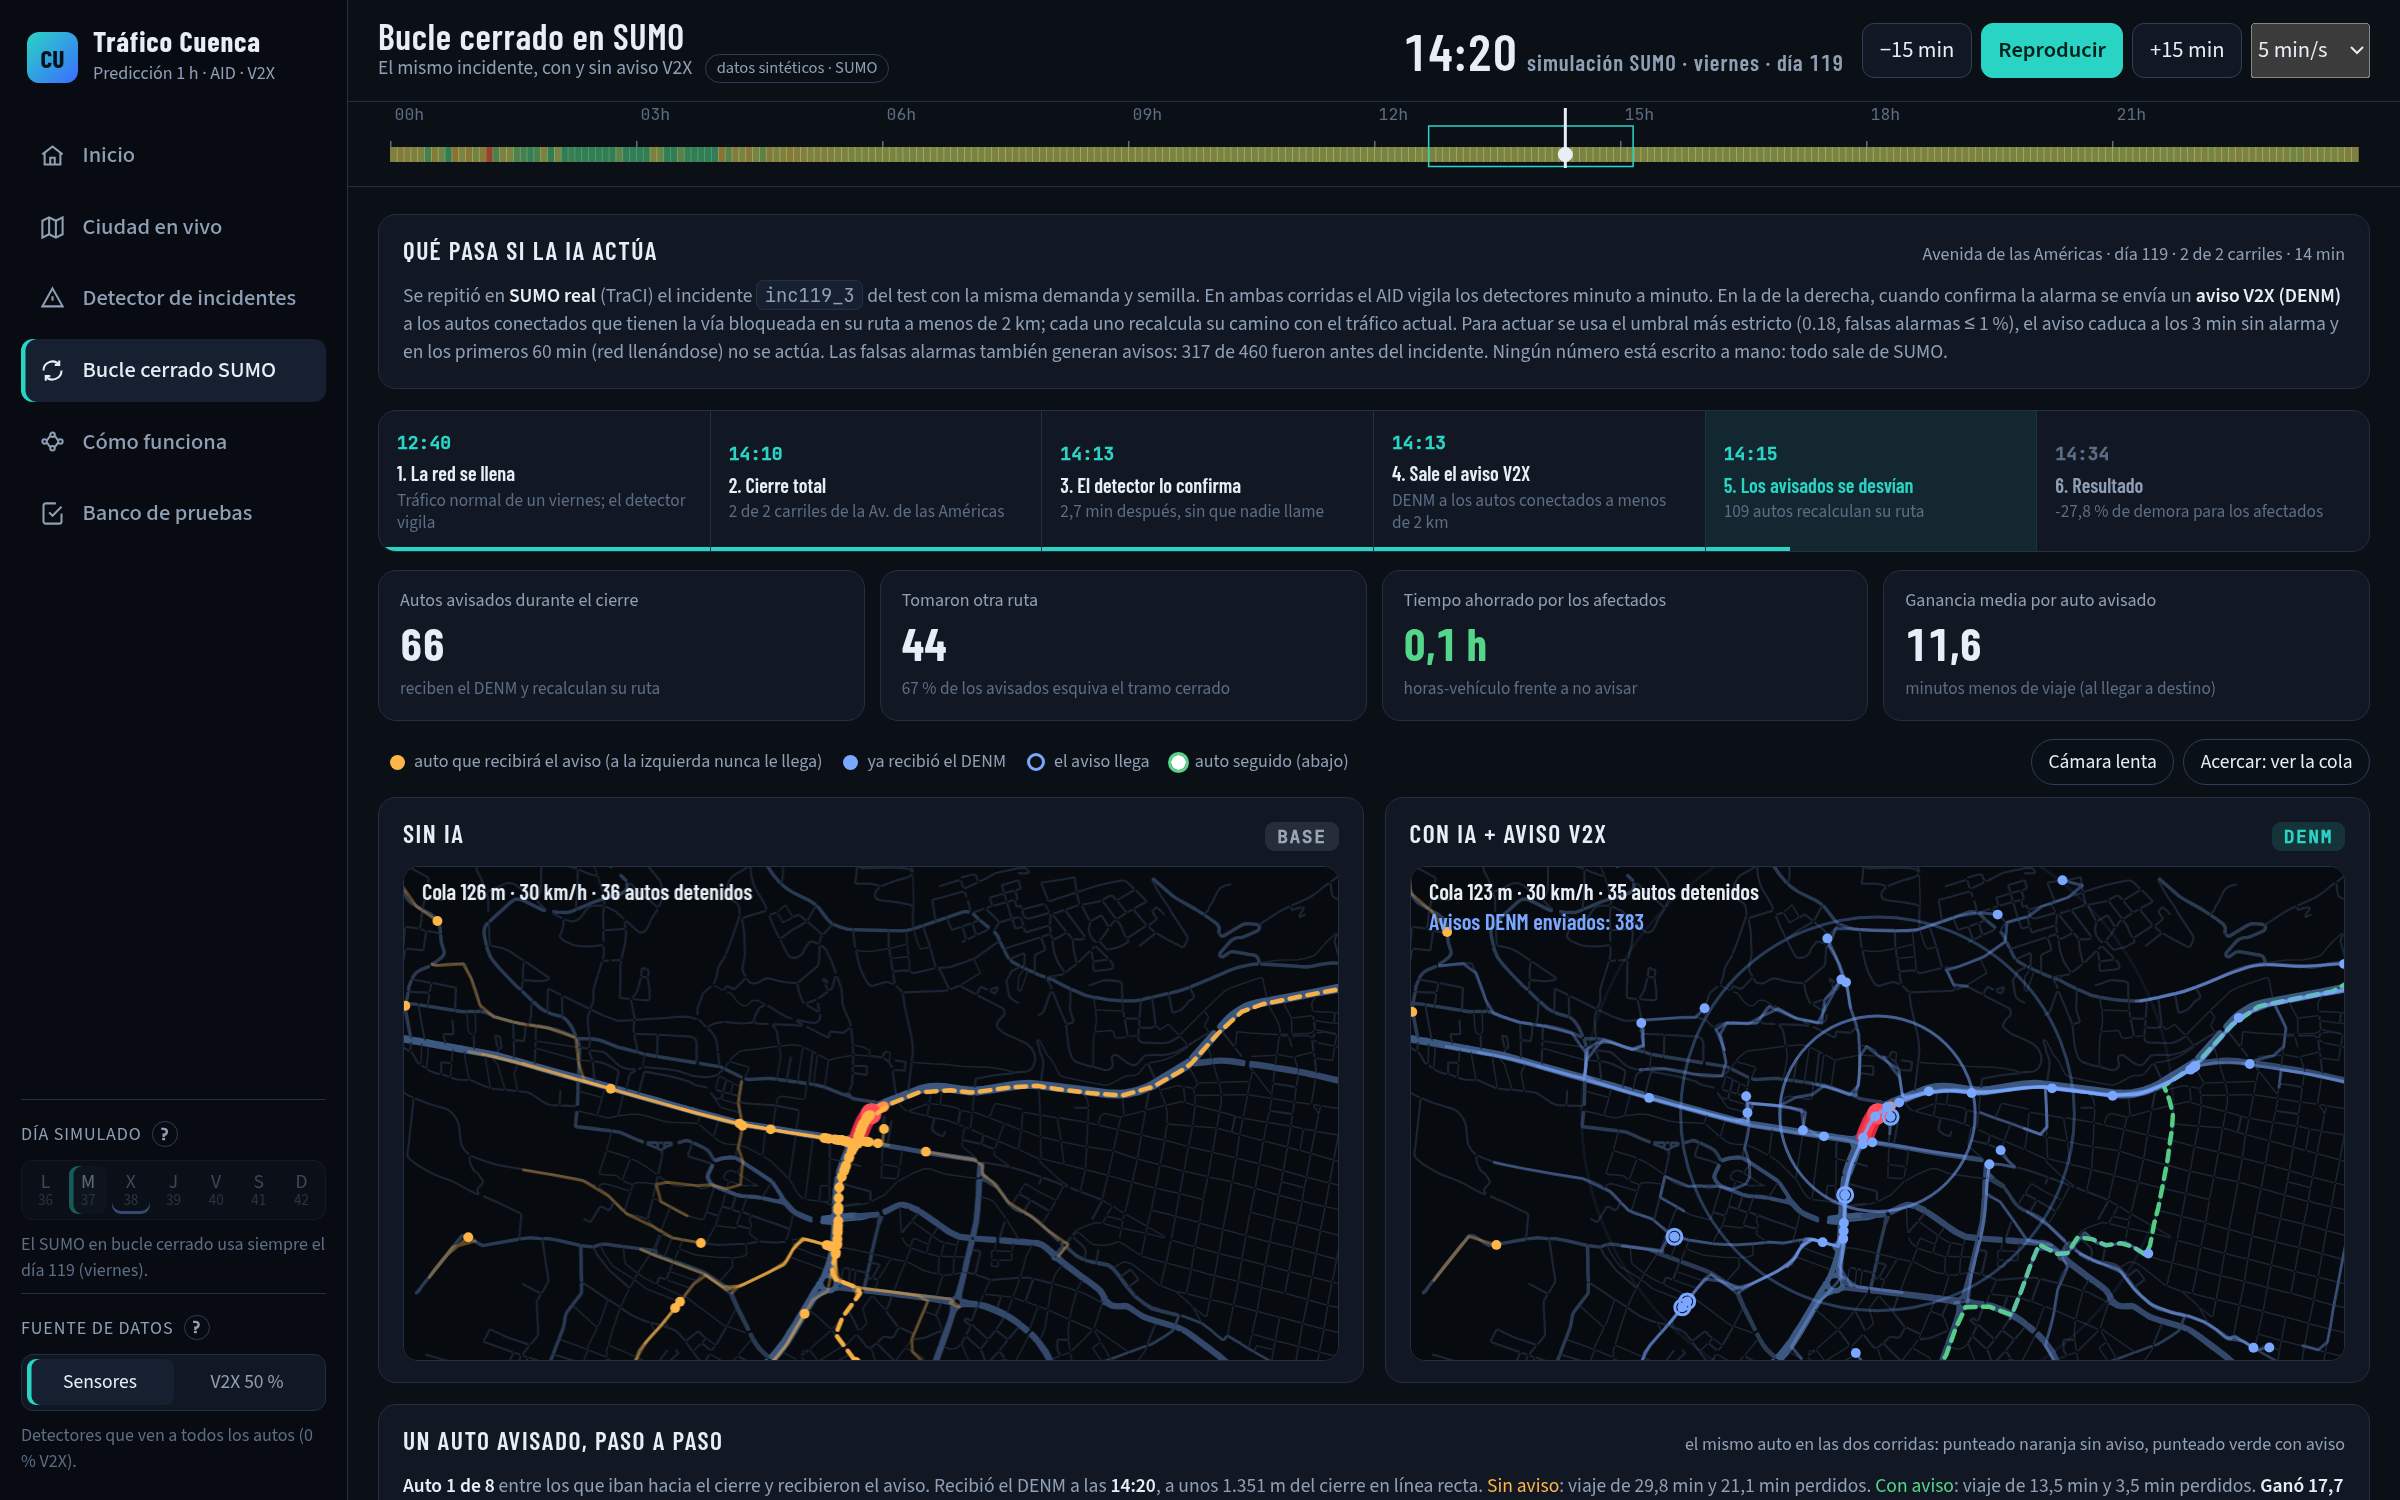
\includegraphics[height=.76\textheight]{dash_sil.png}\\[2pt]
{\scriptsize\color{gris}Cierre total de la Av. de las Américas, día 119, 14:10. Izquierda: sin aviso. Derecha: con la IA y avisos V2X. Datos sintéticos (SUMO).}
\end{frame}

% ================= FERNANDO
\begin{frame}{Resultados frente a la línea base}
\footnotesize
\centering
\begin{tabular}{@{}llll@{}}
\toprule
Parte & Línea base & Este proyecto & Cambio \\
\midrule
Predicción a 1 h (MAE) & promedio histórico 3,16 km/h & \textbf{1,82 km/h} (V2X: 1,86) & \textcolor{verde2}{\textbf{−43 \%}} \\
 & persistencia 3,75 km/h & & \textcolor{verde2}{−51 \%} \\
Predicción, día de lluvia & promedio histórico 5,40 km/h & \textbf{1,78 km/h} & \textcolor{verde2}{\textbf{−67 \%}} \\
\midrule
Detector (con cola detectados) & azar con las mismas alarmas 14 \% & \textbf{90 \%} & \textcolor{verde2}{\textbf{×6}} \\
Detector, falsas alarmas & meta 3–5 \% & 1,9–4,4 \% & \textcolor{verde2}{en la meta} \\
Detector, minutos a la alarma & meta < 5 min & 4,5 min (normales: 7,3) & \textcolor{rojo}{parcial} \\
\midrule
Aviso V2X: demora de afectados & sin aviso 314 s & \textbf{227 s} & \textcolor{verde2}{\textbf{−27,8 \%}} \\
Aviso V2X: demora de la red & sin aviso 153 s & 140 s & \textcolor{verde2}{−8,1 \%} \\
\bottomrule
\end{tabular}

\vspace{8pt}
{\scriptsize Test medido una sola vez, en días que los modelos nunca vieron. \PruebasOk{} de \PruebasTotal{} pruebas automáticas verifican cada cifra.}\\[2pt]
\sint
\end{frame}

% ================= KARLA
\begin{frame}{Conclusiones}
\begin{columns}[T]
\begin{column}{.32\textwidth}
\begin{block}{Predecir}
\small 1,82 km/h de error a 1 hora, \alert{43 \% menos} que lo habitual; igual con solo 50 \% de autos V2X.
\end{block}
\end{column}
\begin{column}{.32\textwidth}
\begin{block}{Detectar}
\small \alert{9 de cada 10} accidentes con cola, en 4,5 min; el azar, 1 de cada 7.
\end{block}
\end{column}
\begin{column}{.32\textwidth}
\begin{block}{Avisar}
\small \alert{−28 \%} de demora para los autos que iban al cierre y −8 \% en toda la red.
\end{block}
\end{column}
\end{columns}
\vspace{14pt}
\begin{center}
\alert{El lazo completo funciona, y el dato real de la EMOV entra sin cambiar el código.}\\[6pt]
{\small\color{gris}Siguiente paso: un detector más rápido en días tranquilos y más accidentes en el bucle cerrado.}
\end{center}
\end{frame}

{\setbeamercolor{background canvas}{bg=verde}
\begin{frame}[plain]
\centering
\vspace{1.5cm}
{\color{white}\fontsize{34}{36}\selectfont\bfseries ¡Gracias!}\\[10pt]
{\color{white}\large ¿Preguntas?}\\[18pt]
{\color{white!80!verde}\small Angel Apolo · Fernando Terán · Stalyn Ochoa · Karla Barrera}
\end{frame}}

\end{document}
